% !TEX TS-program = pdflatexmk
\documentclass{./packages/optica-article}

\graphicspath{{images/}{practica1/images}}

\journal{opticajournal}

\usepackage{csvsimple}
\usepackage{siunitx}
\usepackage{physics}
\usepackage{booktabs}
\usepackage{tikz}
\usetikzlibrary{positioning}

\tikzset{>=stealth}

% cref instead of ref
\usepackage{cleveref}

\newcommand{\sinc}{\textrm{sinc}}
\newcommand\conv{\circledast}

% Set the article type
\articletype{Research Article}

\begin{document}

\title{Caracterización de sistemas de formación de imágenes}

\author{Adriana Mamani Lazarte\authormark{1} Alex G. Recuenco\authormark{1}, and Carlos España Castaño\authormark{1}}

\address{\authormark{1}Universidad Complutense de Madrid, Madrid, PC 28040, España}

\section{Introducción}
En esta práctica vamos a caracterizar un sistema de formación de imágenes mediante la determinación experimental de su función de transferencia de modulación (MTF). Para ello utilizaremos un método directo (el test de barras) y un método indirecto (el test de borde).


\section{TODO: SETUP, or whichever way you call it}

El sistema cuya MTF mediremos consiste en un objetivo de microscopio con apertura numérica $NA = 0,25$ y un aumento $10X$ (F10), y una cámara CCD con un tamaño de píxel de $s=4,65 \mu m$. Las imágenes captadas por la cámara se visualizarán en la pantalla del PC.

\subsection{Fundamento teórico}

\begin{itemize}
	\item Poner referencias
	\item ?`Tenemos que explicar de donde viene esto?
\end{itemize}


\subsection{Medida de MTF mediante el test de barras (método directo)}

\begin{itemize}
	\item Poner un ejemplo de imagen, y un ejemplo de grafica de contraste, con los $y_{\max/\min}$ y $x_{\max/\min}$

\end{itemize}

\subsection{Medida de la MTF mediante el test de borde (método indirecto)}
\section{Resultados experimentales}

\subsection{Medida de la MTF mediante el test de barras (método directo)}

Utilizamos el test USAF 1951 (Fig.~\ref{fig:usaf1951}):

\begin{figure}[htbp]
	\centering
	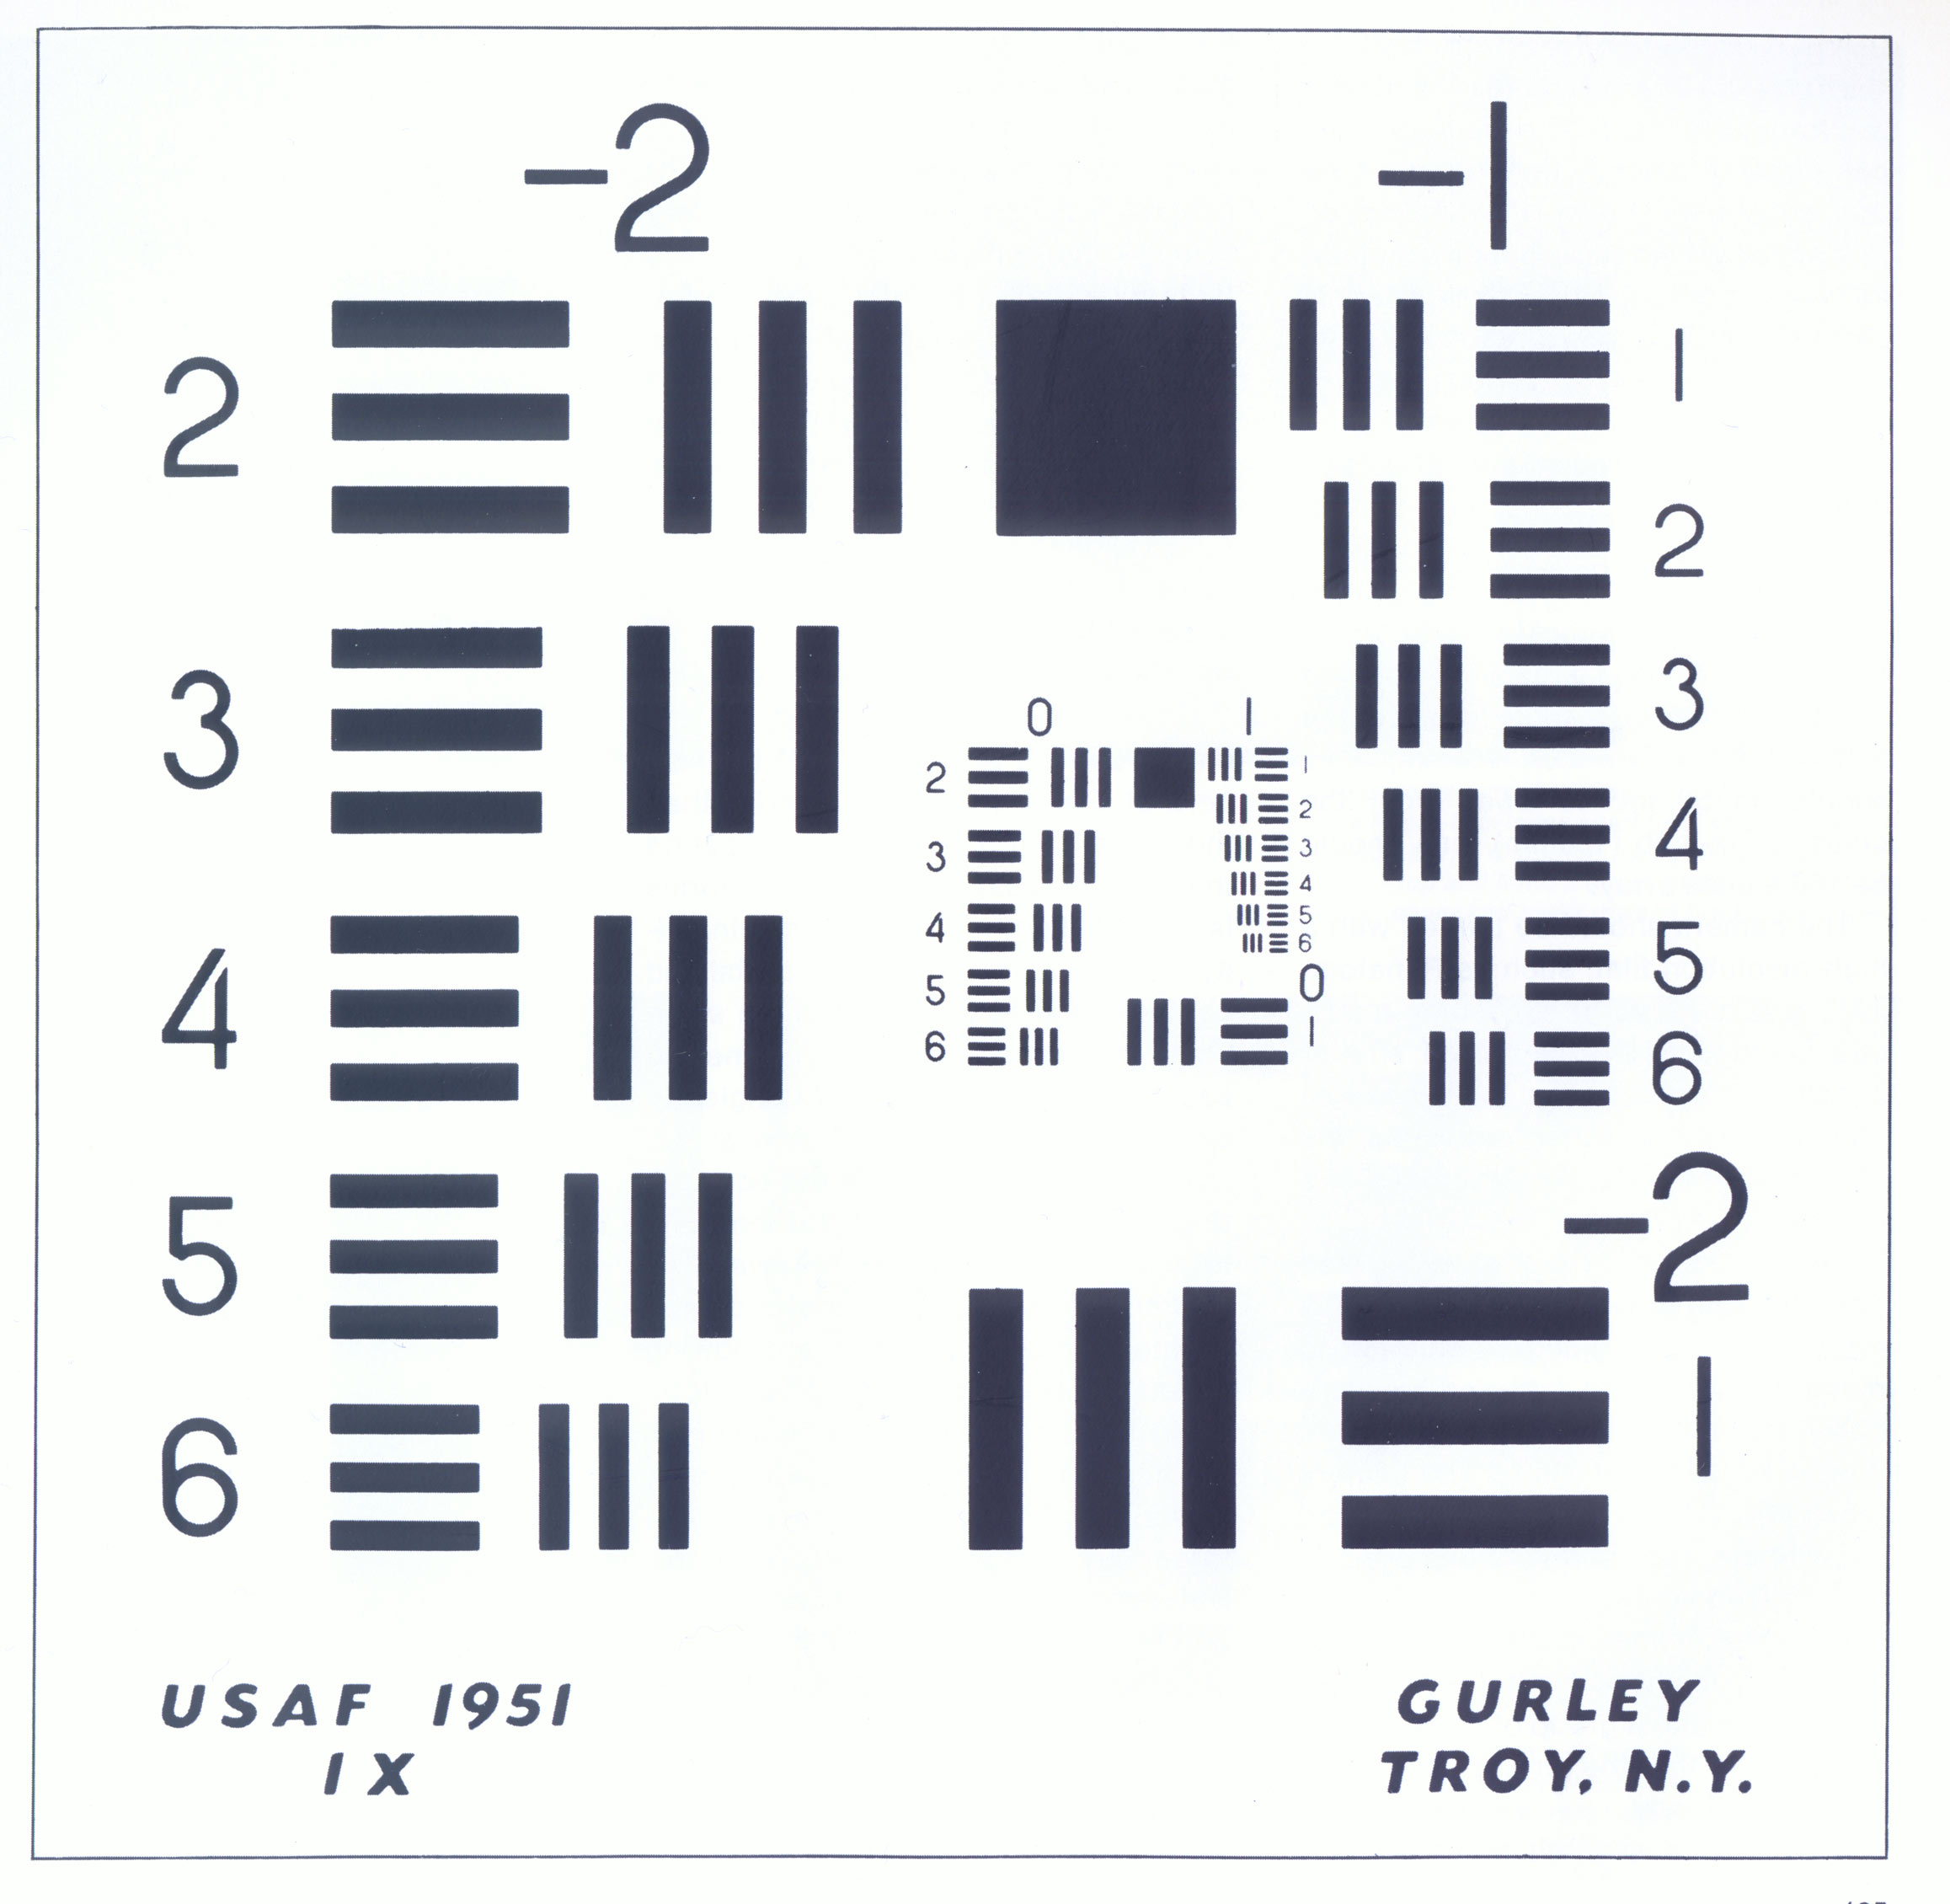
\includegraphics[scale=0.05]{testusaf1951}
	\caption{Test USAF 1951}\label{fig:usaf1951}
\end{figure}

En la tabla~\ref{table:perfilintensidad} se recogen medidas tomadas del perfil de intensidad para distintos conjuntos de barras.

\begin{table}[p]
	\centering
	\csvautotabular[
		table head=\toprule%
		Barras & $y_{\min} (px)$ & $y_{\max} (px)$ & Contraste & $x_{\min} (px)$ & $x_{\max} (px)$ & N Periodos & periodo (px) &  $\flatfrac{\textrm{ciclos}}{\textrm{mm}}$%
		\\\midrule%
	]{practica1/MTF/Profiles.csv}
	\caption{Datos del perfil de intensidad. $y$: intensidad. $x$: distancia en píxeles. El contraste se ha obtenido a partir de la eq. \ref{eq:contraste}. la frequencia se ha obtenido a traves de la eq. \ref{eq:frecuencia}}%
	\label{table:perfilintensidad}
\end{table}

El contraste se ha obtenido a partir de la expresión
\nopagebreak
\begin{equation}
	C = \frac{y_{\max} - y_{\min}}{y_{\max} + y_{\min}}.
	\label{eq:contraste}
\end{equation}

La frecuencia, se calcula como:

\begin{equation}
	\nu = \frac{1825}{T}\ \textrm{ciclos/mm},\quad\textrm{TODO: QUE es 1825??}
	\label{eq:frecuencia}
\end{equation}

Donde el periodo, $T$, se obtiene dividiendo la diferencia $x_{\max} - x_{\min}$ entre el número de periodos en ese intervalo.

TODO: Incluir grafica de ejemplo, indicando como se obtinee

\subsection{Medida de la MTF mediante el test de borde (método indirecto)}

\section{Cuestiones}

\subsection{Sea $H_{c}(u)$ la función de transferencia de un sistema para luz coherente. Escribir la relación entre $H_{c}(u)$ y la función de transferencia del mismo sistema para luz incoherente, $H_{i}(u)$.}

Cuando la luz incidente coherente incide, la resolución es lineal en su amplitud compleja. Sin embargo, cuando la iluminación es incoherente, la iluminación es linear en intensidad. Por ello, en el caso ideal donde la correlación de fase es zero para distintas posiciones, se obtiene que \cite[p.~132--134]{goodman1996introduction}.

\begin{equation}
	I_{i}(u,v) = \kappa \iint_{-\infty}^{\infty}\abs{h(u - \xi, v- \eta)}^{2} I_{g}(\xi, \eta) \dd \xi \dd \eta
\end{equation}

Por lo tanto, la funcion $H_{i}(u)$ se puede obtener con el schema descrito en Fig. \ref{fig:transformacion}. Basicamente, haciendo la transformación inversa para obtener $h_{c}$, luego multiplicando esta con su conjugada, obteniendo $h_{i}$, donde $i$ denota intensidad. Y al realizar la transformada inversa obtenemos el resultado.

\begin{align}
H_{i}(u) 
	&= TF\{h_i\} 
	= TF\left\{ h_{c} \cdot h^{*}_{c}\right\}
	= TF\left\{ h_{c} \cdot h^{*}_{c}\right\} 
	= TF\left\{ TF^{-1}\{H_{c}\} \cdot {TF^{-1}\{H_{c}\}}^{*}\right\} 
	\\
 &= H_{c} \conv H^{*}_{c}
\end{align}

\begin{figure}[htpb]
\begin{center}
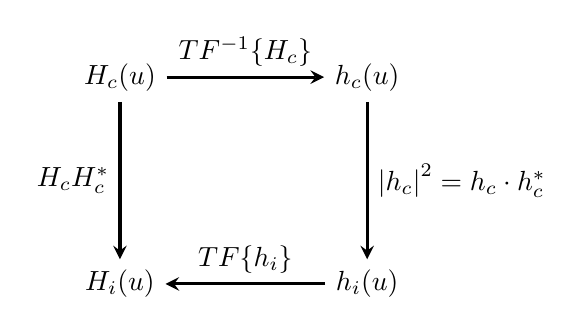
\begin{tikzpicture}[line width=0.4mm]

\def \n {5}
\def \radius {3cm}
\def \margin {8} % margin in angles, depends on the radius

\node (H) at (0,0) {$H_{c}(u)$};
\node[right=2cm of H] (h) {$h_{c}(u)$};
\node[below=2cm of h] (hi) {$h_{i}(u)$};
\node[below=2cm of H] (Hi) {$H_{i}(u)$};
\draw[->] (H) -- (h) node[pos=0.5, anchor=south] {$TF^{-1}\{H_{c}\}$};
\draw[->] (h) -- (hi) node[pos=0.5, anchor=west] {$\abs{h_{c}}^{2} = h_{c} \cdot h^{*}_{c}$};
\draw[->] (hi) -- (Hi) node[pos=0.5, anchor=south] {$TF\{h_{i}\}$};
\draw[->] (H) -- (Hi) node[pos=0.5, anchor=east] {$H_{c} \conv H^{*}_{c}$};
\end{tikzpicture}
\end{center}
\caption{Diagrama TODO, describirlo mejor}
\label{fig:transformacion}
\end{figure}

\subsection[]{Para un sistema parecido al usado en la práctica:
	\begin{enumerate}
		\item Estimar la frecuencia de corte de la cámara CCD, $u_{c}^{(CCD)}$, en líneas por milímetro.
		\item Estimar la frecuencia de corte $u_{c}^{(Obj)}$ del objetivo $10\times$ para luz incoherente (la longitud de onda media $\lambda=500\,\unit{\nano\metre}$).
		\item Tomando estos valores y suponiendo que la PSF del objetivo y de la cámara se aproximan por la función $|\sinc(ax)|^2$, dibujar la MTF de cada uno de los elementos y del sistema compuesto.
	\end{enumerate}}



\subsection{Aplicar usando el plugin Deconvolutionlab2 y Image J dos métodos de convolución: Regularized Inverse Filter y Richardson-Lucy a una imagen test obtenida por un sistema con una PSF conocida y diferentes tipos de ruido: Guass y Poisson.}


%%%%%%%%%% If using BibTeX:
\bibliography{bibliography}

\end{document}
